\documentclass[submission, LectureNotes]{SciPost}

\usepackage{amsmath, amssymb}
\usepackage{graphicx}
\usepackage{bm}
\usepackage{color}
\usepackage{enumerate}
\usepackage{physics}
\usepackage{siunitx}
\usepackage{listings}
\usepackage{pythonhighlight}
\usepackage{exercise}

\definecolor{LightGray}{rgb}{0.9, 0.9, 0.9}

\newcommand{\hatd}{{\ensuremath{\hat{d}}}}
\newcommand{\hatc}{{\ensuremath{\hat{c}}}}
\newcommand{\Ne}{{\ensuremath{N_\mathrm{e}}}}
\newcommand{\bk}{\ensuremath{{\bf k}}}
\newcommand{\br}{\ensuremath{{\bf r}}}

\newcommand{\bx}{\bm{x}}
\newcommand{\by}{\bm{y}}
\newcommand{\bS}{S}
\newcommand{\bU}{U}
\newcommand{\bV}{V}
\newcommand{\bK}{K}
\newcommand{\brho}{\bm{\rho}}
\newcommand{\bG}{\bm{G}}
\newcommand{\wmax}{\ensuremath{{\omega_\mathrm{max}}}}
\newcommand{\Nband}{\ensuremath{{N_\mathrm{band}}}}
\newcommand\cee{\mathrm{c}}%
\newcommand\cdag{\mathrm{c}^\dagger}%
\newcommand\ee{\mathrm{e}}%
\newcommand\ii{\mathrm{i}}%
\newcommand\iv{\ii\nu}%
\newcommand\iw{\ii\omega}%
\newcommand\iW{\ii\Omega}%
\newcommand\WW{\mathcal{W}}
\newcommand\FF{\mathrm{F}}
\newcommand\BB{\mathrm{B}}
\newcommand\Fbar{\mathrm{\bar F}}
\newcommand\Bbar{\mathrm{\bar B}}
\newcommand{\GW}{{\ensuremath{GW}}}
\newcommand{\tauk}{\ensuremath{\bar{\tau}^\alpha_k}}
\newcommand{\taukF}{\ensuremath{\bar{\tau}^\mathrm{F}_k}}
\newcommand{\wk}{\ensuremath{\bar{\omega}^\alpha_k}}

\newcommand{\wkF}{\ensuremath{\bar{\omega}^\mathrm{F}_k}}

\newcommand{\hatFmat}{\hat{\mathbf{F}}}
\newcommand{\Fmat}{{\mathbf{F}}}

\newcommand{\KF}{\ensuremath{K^\mathrm{F}}}
\newcommand{\KB}{\ensuremath{K^\mathrm{B}}}
\newcommand{\kF}{\ensuremath{k^\mathrm{F}}}
\newcommand{\kB}{\ensuremath{k^\mathrm{B}}}
\def\deltaB{\delta_{\alpha, \mathrm{B}}}
\def\deltaF{\delta_{\alpha, \mathrm{F}}}

\begin{document}

\begin{center}{\Large \textbf{
    Numerical recipes for many-body physics
}}\end{center}

\begin{center}
Hiroshi Shinaoka\textsuperscript{1*},
\end{center}

\begin{center}
{\bf 1} Department of Physics, Saitama University, Saitama 338-8570, Japan
\\
* h.shinaoka@gmail.com
\end{center}

\begin{center}
\today
\end{center}


\section*{Abstract}
This lecture note reviews ....

\vspace{10pt}
\noindent\rule{\textwidth}{1pt}
\tableofcontents\thispagestyle{fancy}
\noindent\rule{\textwidth}{1pt}
\vspace{10pt}

\section{Introduction}

\clearpage
\section{Green's functions}
\subsection{Fermionic and bosonic correlation functions}
%One-particle Green's functions represent one-particle responses of an equilibrium state.
We define retarded/advanced/imaginary-time correlation functions as
\begin{align}
	G^\mathrm{R}(t-t') &= -\ii \theta(t-t')\expval{A(t)B(t')\mp B(t')A(t)},\\
	G^\mathrm{A}(t-t') &= -\ii \theta(t'-t)\expval{A(t)B(t')\mp B(t')A(t)},\\
	G(\tau-\tau') &= -\theta(\tau-\tau')\expval{A(\tau)B(\tau')} \mp \theta(\tau'-\tau) \expval{B(\tau')A(\tau)}.
\end{align}
The operators $A$ and $B$ are either fermionic or bosonic.
The signs $\mp$ are for bosons and fermions, respectively.
$\expval{\cdots}$ represents statistical average in the the grand canonical ensamble.
%The symbols $a$ and $b$ denote spin orbitals,
%while $c_a$ and $c^\dagger_b$ denote annihilation and creation operators.
%The first two are defined in real time, while the last one in imaginary time.
%
%These Green's functions 
These real-time/imaginary-time correlation functions are transformed to
real frequency and imaginary (Matsubara) frequencies, respectively:
%For a while, we focus on fermionic Green's functions.
%can be represented in a unified form using Lehmann representation:
\begin{align}
    G^\mathrm{R}(\omega) &= \int_{-\infty}^\infty \dd t e^{\ii\omega t}G^\mathrm{R}(t),\\
    G^\mathrm{A}(\omega) &= \int_{-\infty}^\infty \dd t e^{\ii\omega t}G^\mathrm{A}(t),\\
    G(\iv) &= \int_0^\beta \dd \tau e^{\iv \tau}G(\tau),\label{eq:matsubara-AB}
\end{align}
where Matsubara frequencies are given by $\nu = 2n\pi/\beta$ and $\nu = (2n+1)\pi/\beta$ for bosons/fermions, respectively ($n\in \mathbb{Z}$).
We defined $\beta = 1/T$ ($k_\mathrm{B}=1$).
%These correlation functions be analytically transformed to each other as we will see later.

In the grand canonical ensemble, $G(\iv)$ has the Lehmann representation:
\begin{align}
    G_{AB}(\iv) &= \int \dd \omega \frac{\rho_{AB}(\omega)\omega^{\delta_{\alpha,\mathrm{B}}}}{\iv - \omega},\\
    \rho_{AB}(\omega) &\equiv -\frac{1}{\pi\omega^\delta_{\alpha,\mathrm{B}}} \imaginary G_{AB}(\omega + 0^+)\\
    & = \frac{1}{Z}\sum_{mn}(e^{-\beta E_n} \mp e^{-\beta E_m})
    \mel{n}{A}{m}\mel{m}{B}{n}
    \delta(\omega - (E_m-E_n)),\label{eq:matsubara-lehmann}
\end{align}
where
$n$, $m$ run over all eigenstates of the system ($E_{m/n}$ denotes an eigenvalue).
We introduced the extra factor $\omega^{\delta_{\alpha,\mathrm{B}}}$ for bosons ($\alpha$ represents the staistics),
whose reasoning will be explained later.

Using Eq.~\eqref{eq:matsubara-lehmann},
we can analytically continue $G(\iv)$ to the whole complex plane as $G(z)$ for $z\in \mathbb{C}$.
Note that there are poles or a branch cut on the real axis.
%Using $G_{AB}(z)$, the real-frequency and imaginary-frequency (Matsubara) Green's funcitons are analytically continued as
The advanced and retarded Green's functions are given by the value of $G_{AB}(z)$ above/below the real axis as
\begin{align}
    G^\mathrm{R}_{AB}(\omega) &= G_{AB}(\omega+\ii 0^+),\\
    G^\mathrm{A}_{AB}(\omega) &= G_{AB}(\omega+\ii 0^-).
\end{align}
Due to the branch cut on the real axis, $G^\mathrm{R}_{AB}(\omega) \neq G^\mathrm{A}_{AB}(\omega)$ in general.

At high frequencies, $G(\iv)$ decays in power.
Applying partial integration recursively to Eq.~\eqref{eq:matsubara-AB},
we obtain its high frequency expansion,
\begin{align}
    G_{AB}(\iv) &= 
    \frac{c^{(1)}_{AB}}{\iv} +
    \frac{c^{(2)}_{AB}}{(\iv)^2} +
    \frac{c^{(3)}_{AB}}{(\iv)^3} + \cdots,
\end{align}
where
\begin{align}
    c^{(m)}_{AB} &= (-1)^{m} \qty(G_{AB}^{(m-1)}(0^+) - G_{AB}^{(m-1)}(0^-)).
\end{align}
In particular, one can show
\begin{align}
   c^{(1)}_{AB} &= \poissonbracket{A}{B}.
\end{align}


\subsection{Fermionic one-particle Green's function}
We focus on the fermionic cases where $A$ and $B$ are annihilation and creation operators of fermions, respectively.
In such cases, the correlation is called ``(one-particle) Green's function''.
The Lehmann representation of the Green's function reads
\begin{align}
    G_{ab}(\iv) &= \int \dd \omega \frac{\rho_{ab}(\omega)}{\iv - \omega},\\
    \rho_{AB}(\omega) &\equiv -\frac{1}{\pi} \imaginary G_{ab}(\omega + 0^+)\\
    & = \frac{1}{Z}\sum_{mn}(e^{-\beta E_n} + e^{-\beta E_m})
    \mel{n}{c^\dagger_a}{m}\mel{m}{c_b}{n}
    \delta(\omega - (E_m-E_n)),\label{eq:matsubara-g-lehmann}
\end{align}
where $a$ and $b$ denote spin orbitals.

Applying partial integration recursively to Eq.~\eqref{eq:matsubara-AB},
we obtain a high frequency expansion of the Green's function,
\begin{align}
    G_{ab}(\iv) &= 
    \frac{c^{(1)}_{ab}}{\iv} +
    \frac{c^{(2)}_{ab}}{(\iv)^2} +
    \frac{c^{(3)}_{ab}}{(\iv)^3} +
    O\qty(\frac{1}{(\iv)^4}),
\end{align}
where
\begin{align}
    c^{m}_{ab} &= (-1)^{m} \qty(G_{ab}^{(m-1)}(0^+) - G_{ab}^{(m-1)}(0^-)).
\end{align}
In particular, one can show
\begin{align}
   c^{0}_{ab} &= \poissonbracket{c_a}{c^\dagger_b} = \delta_{ab}.
\end{align}

This clearly indicates that the Green's function has a discontinuity at $\tau=0,\pm \beta, \pm 2\beta$ for $a=b$.
At these points, the off-diagonal components ($a\neq b$) have a slope discontinuity or a discontinuity in higher-order derivatives.
For $0 <\tau < \beta$, the Green's function is a smooth and analytic function.
%
%The sum rules is followed by $c_{ab}^1 = \delta_{ab}$.
%The slow power-law decay originates from the discontinuity of $G(\tau)$ and its derivatives at $\tau=0,\pm \beta, \pm 2\beta, \cdots$.
%\
%
%Below, we summarize the analytic properties of the fermionic Green's function.
%
%Pros:
%\begin{itemize}
    %\item $G(\tau)$ is a smooth function for $0<\tau<\beta$.
    %\item Good resoluation at low frequencies
%\end{itemize}
%
%Cons:
%\begin{itemize}
    %\item $G(\tau)$ is not continuous at $\tau=0,\pm \beta, \cdots$, leading to the nesscecity of cumbersome numerical tricks.
    %\item Numerical analytic continuation to high frequencies is not stable.
%\end{itemize}

\subsection{Example: Hubbard atom}
We consider the single-orbital fermionic Hubbard atom at half filling:
\begin{align}
   \mathcal{H} &= U n_\uparrow n_\downarrow - \mu (n_\uparrow + n_\downarrow),
\end{align}
where $\mu= U/2$ and $U>0$.
By simple calculations, one obtains
\begin{align}
    G_{\sigma\sigma'}(z) &= \frac{1}{2}\qty(\frac{1}{z-U/2} + \frac{1}{z+U/2})\delta_{\sigma\sigma'},\label{eq:gz-hubbard-atom}
\end{align}
where $\sigma$ and $\sigma'$ are spin indices.
This can be transformed to the imaginary-time domain as
\begin{align}
    G_{\sigma\sigma'}(\tau) &= -\frac{1}{2}
    \qty(
        \frac{e^{-\tau U/2}}{1+e^{-\beta U/2}} +
        \frac{e^{\tau U/2}}{1+e^{\beta U/2}}
    )\delta_{\sigma\sigma'}\label{eq:gtau-hubbard-atom}
\end{align}
for $0 < \tau<\beta$.

%\subsection{Exercise 1}
\begin{Exercise}[label=ex1]
Plot Eqs.~\eqref{eq:gz-hubbard-atom} and \eqref{eq:gtau-hubbard-atom} for a typical value of $\beta$.
You will see that $G(\tau)$ changes very rapidly around $\tau=0$ and $\beta$ at large $\beta$.
Due to the sum rule and the half-filling condition,
$G_{\sigma\sigma'}(0^+)=G_{\sigma\sigma'}(\beta+0^-) = -1/2$.
On the other hand, $G(\iv)$ decays only algebraically at high frequencies.
Your plot should look like Figs.~\ref{fig:gtau-hubbard-atom} and~\ref{fig:giv-hubbard-atom}.
\end{Exercise}

\begin{figure}
    \centering
    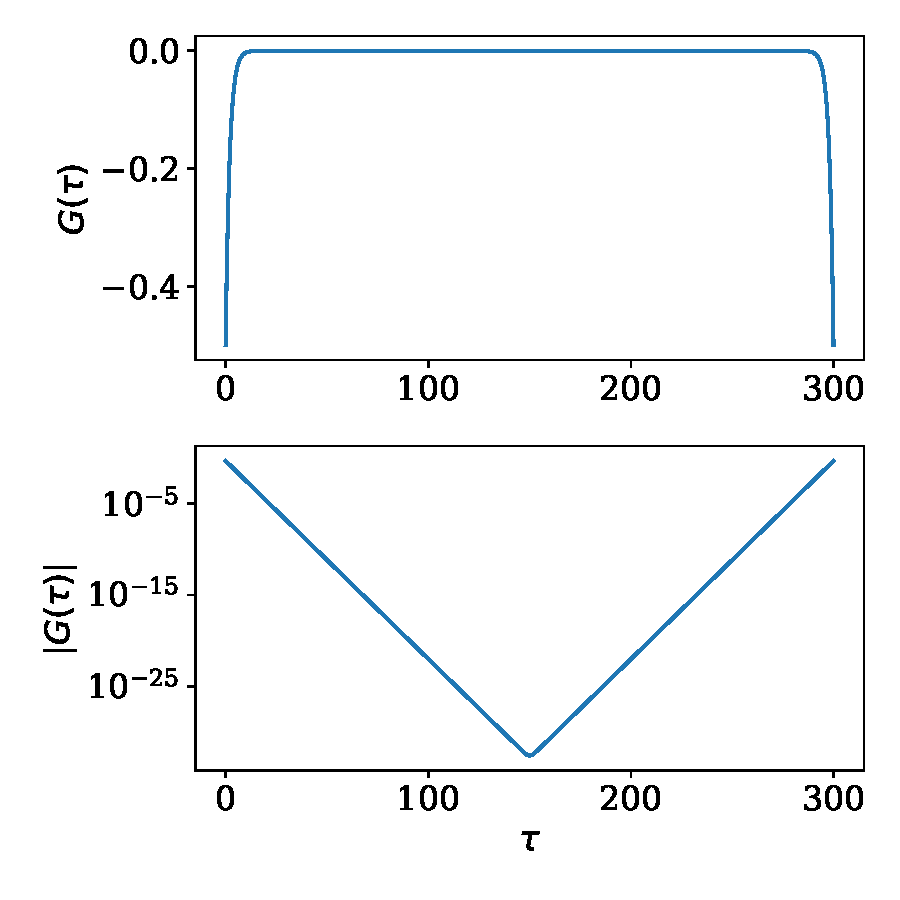
\includegraphics[width=0.5\columnwidth]{gtau_hubbard_atom.pdf}
    \caption{$G(\tau)$ computed for the Hubbard atom with $U=1$ and $\beta=300$.}
    \label{fig:gtau-hubbard-atom}
\end{figure}
\begin{figure}
    \centering
    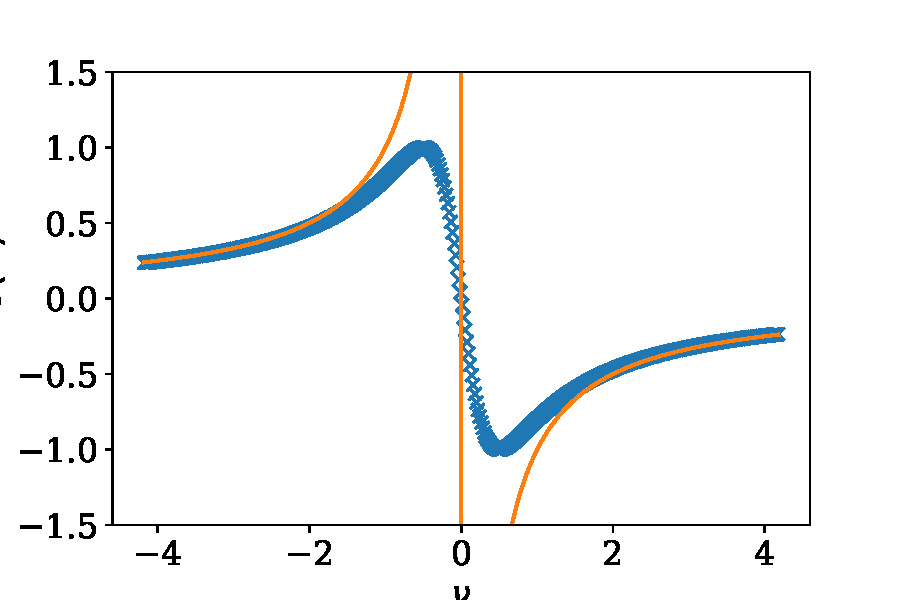
\includegraphics[width=0.5\columnwidth]{giv_hubbard_atom.pdf}
    \caption{$G(\iv)$ computed for the Hubbard atom with $U=1$ and $\beta=300$. The solid curve denotes $-1/\nu$.}
    \label{fig:giv-hubbard-atom}
\end{figure}

\begin{Exercise}
Derive Eq.~\eqref{eq:gtau-hubbard-atom} from Eq.~\eqref{eq:gz-hubbard-atom} using 
the formula
\begin{align}
   T\sum_{\nu} \frac{e^{-\iv\tau}}{\iv - \epsilon} &= - \frac{e^{-\epsilon\tau}}{1+e^{-\beta\epsilon}}.\label{eq:single-pole-ft}
\end{align}
\end{Exercise}

\begin{Exercise}[label=ex:native-inverse-transform]
Please numerically check how $G(\tau)$ of the Hubbard atom behaves near $\tau=0$ if we truncate the summation in Eq.~\eqref{eq:single-pole-ft} at some frequency.
The result should look like Fig.~\ref{fig:naive-inverse-transform-hubbard-atom}.
\end{Exercise}

\begin{figure}
    \centering
    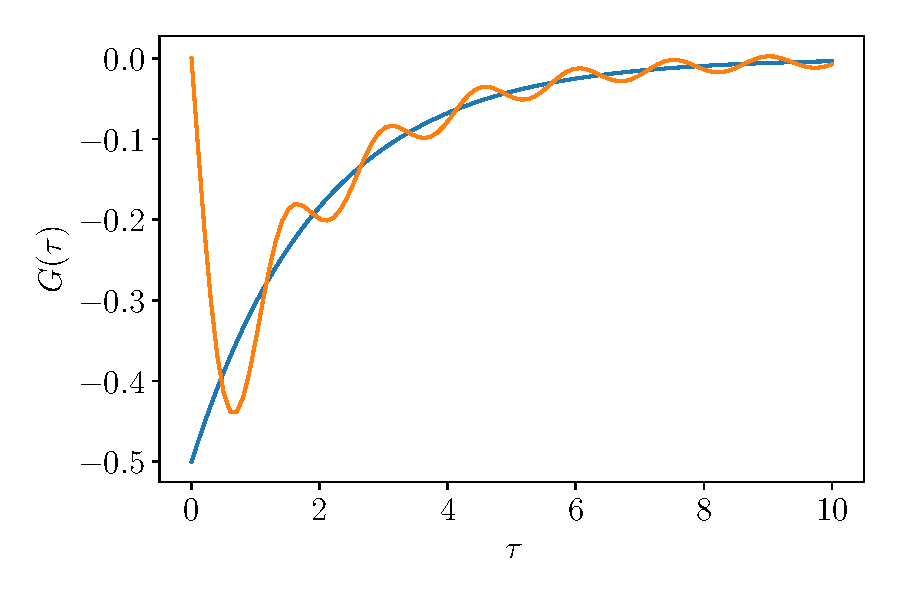
\includegraphics[width=0.5\columnwidth]{naive_inverse_transform_hubbard_atom.pdf}
    \caption{Naive inverse transform of $G(\iv)$ for the Hubbard atom with $U=1$ and $\beta=300$. We used 200 positive Matsubara frequencies.}
    \label{fig:naive-inverse-transform-hubbard-atom}
\end{figure}


\clearpage
\section{Conventional approaches}
\subsection{Uniform mesh}
Due to the algebraic decay of $G(\iv)$ and the strong $\tau$ dependence of $G(\tau)$ around $\tau=0$,
it is a bit cumbersome to treat the Green's function numerically.
In this section, we explain a conventional way of doing so.

A naive way to store the values of the Green's function numerically is to use uniform meshes in $\iv$ and $\tau$.
Although you will see that this fails at low temperatures later,
it may be instructive to start with the simplest one.
In the imaginary-frequency domain, we use a uniform mesh consisting of the lowest $2N_\nu$ imaginary frequencies:
\begin{align}
&\qty{(2n+1)\pi/\beta~| n=-N_\nu, -N_\nu+1, \cdots N_\nu-2, N_\nu-1}.
\end{align}
In the imaginary-time domain, we use a uniform mesh,
\begin{align}
&\qty{\frac{\beta t}{N_\tau-1}~|~t=0, 1, \cdots, N_\tau-1},
\end{align}
where the two end points are interpreted as $0^+$ and $\beta + 0^-$.

Let us consider to discretize a $G(\tau)$ on the uniform mesh as $G_t$ ($t=0, \cdots, N_\tau-1$).
How many mesh points are sufficient for representing $G(\tau)$ accurately?
We consider the simplest case, i.e. the Hubbard atom Eq.~\eqref{eq:gtau-hubbard-atom}.
In this case, $G(\tau)$ can be approximated around $\tau=0$ as
\begin{align}
    G(\tau) &\propto e^{-\tau U/2}.
\end{align}
This indicates that we must increase the density of the mesh points proportionally with $U$ around $\tau=0$.
Considering the band width of the spectrum is $U$, one can see that $N_\tau$ must increase as $O(\beta \wmax)$ in general cases,
where $\wmax$ is a cutoff frequency of the spectrum: i.e., the spectrum is non-zero only in $[-\wmax, \wmax]$.

\subsection{Interpolation}
Even if $G(\tau)$ is known only on a discrete set of data points,
we may want to evaluate it on arbitrary points.
This can be done by interpolating $G(\tau)$ for $0 < \tau < \beta$.
Popular choices are linear interpolation and cubic spline interpolation.
The linear interpolation fits the data using linear piecewise polynomials
and construct new data points within the range of the known data points.
The cubic spline interpolation uses piecewise polynomials of degree 3.
We demonstrate them for the Hubbard atom in Fig.~\ref{fig:interpolation-gtau}.
One can see that the cubic spline interpolation yields better results.
At an arbitrary point, the interpolation error generally vanishes as $O(h^2)$ and $O(h^4)$
for the linear and cubic spline interpolation methods, respectively,
where $h\equiv \beta/N$ and $N$ is the number of data points.

\begin{Exercise}
    Confirm numerically the scaling of the interpolation error 
    with respect to $h$ for these two interpolation methods.
\end{Exercise}

\begin{figure}
    \centering
    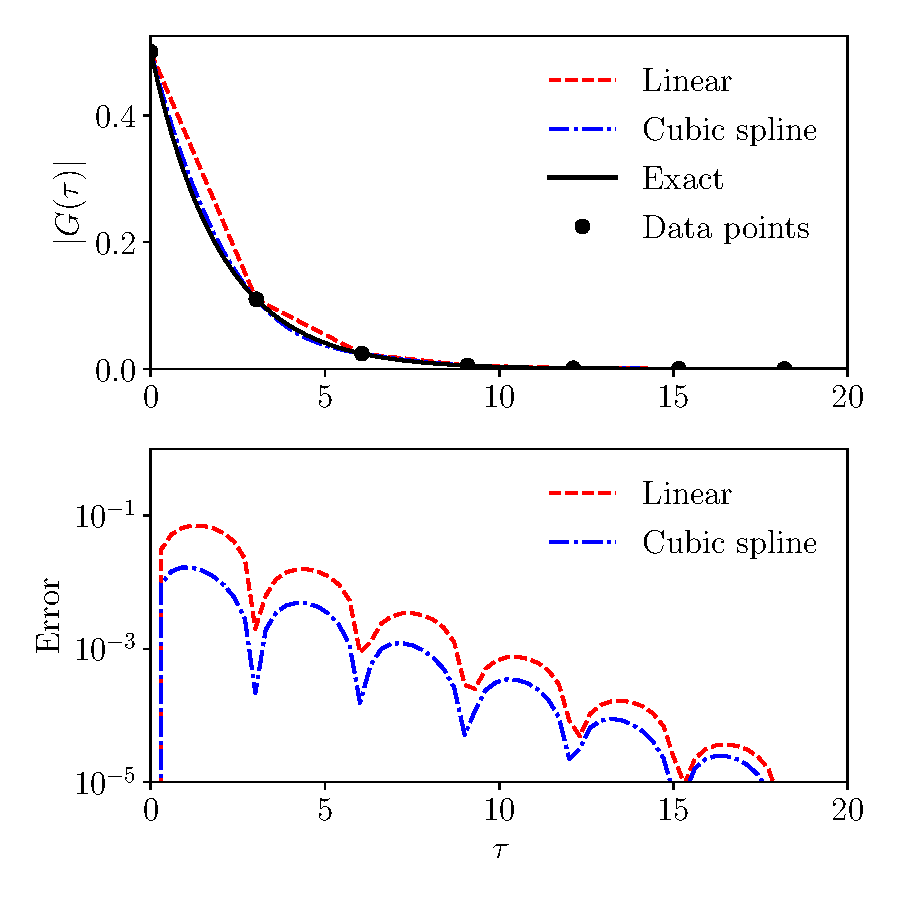
\includegraphics[width=0.8\columnwidth]{interpolation_gtau.pdf}
    \caption{
        Linear and cubic spline interpolations of $G(\iv)$ for the Hubbard atom with $U=1$ and $\beta=300$.
        We used 100 data points.
        }
    \label{fig:interpolation-gtau}
\end{figure}

%
%Thus, we need to \textit{interpolate} the values to evaluate the Green's function in between mesh points.
%An easy way is to use some piecewise polynomial interpolation.
%This is justified by the fact that $G(\tau)$ is a smooth function for $0< \tau<\beta$.

\subsection{Fourier transform}
We explain a naive way to transform numerical data on a uniform mesh in $\tau$ to Matsubara frequencies.
%First, we introduce a quadrature rule for approximating the definite integral of a function.
First, we introduce quadrature rules.
A quadrature rule approximates the definite integral over interval $[-1,1]$ as
\begin{align}
   \int_{-1}^1 f(x) dx \simeq \sum_{i=1}^n w_i f(x_i),
\end{align}
where $w_i$ is a positive weight and $x_i$ is a node.
Different quadrature rules use different choices of weights and nodes.
A popular choice is Gaussian quadrature, which yields accurate results if $f(x)$ can be approximated 
well by a polynomial of degree $2n-1$ or less.

Using your favorite quadrature rule (and interpolation if necessary),
one can Fourier transform numerical data of $G(\tau)$ as
\begin{align}
   G(\iv) &\approx \sum_{i=1}^{n} \tilde{w}_i e^{\iv \tau_i} G(\tau_i),\label{eq:naive-fourier-transform}
\end{align}
where $\tau_i = (x_i+1)\beta/2$ and $\tilde{w}_i=(\beta/2) w_i$.
The RHS of Eq.~\eqref{eq:naive-fourier-transform} converges to the exact value in the limit of $n \rightarrow \infty$.

Figure~\ref{fig:fourier-transform-hubbard-atom} show a numerical demonstration of the Fourier transform using Gauss quadrature.
One can see that the numerical error is very small at low frequencies but the error goes up above some frequency cutoff.

\begin{Exercise}
    Explain why the procedure fails at high frequencies and 
    figure out what determines the cutoff frequency.
    How can we improve on it? (Hint: see Section~\ref{sec:inverse-fourier-transform}).
\end{Exercise}

\begin{figure}
    \centering
    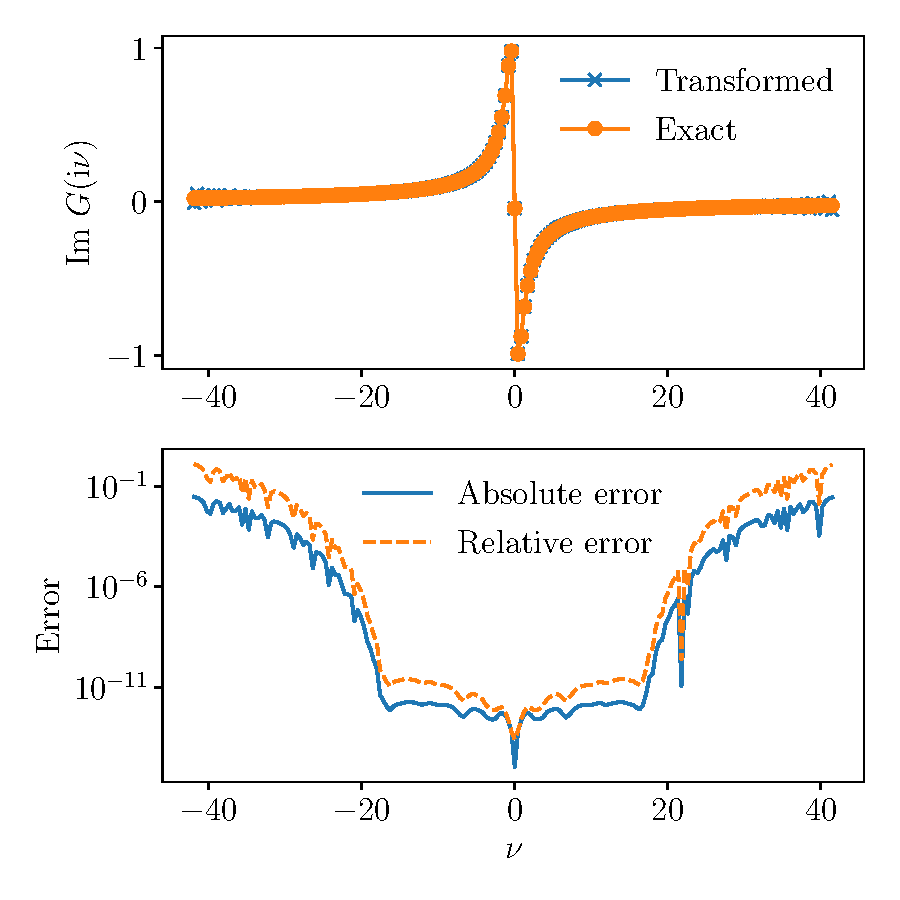
\includegraphics[width=0.8\columnwidth]{fourier_transform_hubbard_atom.pdf}
    \caption{
        Fourier transformation from $G(\tau)$ to $G(\iv)$ for the Hubbard atom with $U=1$ and $\beta=300$.
        We used Gauss quadrature with $n=1000$.
        }
    \label{fig:fourier-transform-hubbard-atom}
\end{figure}

%We first interpolate the numerical value of $G(\tau)$ on a finer mesh in $\tau$, e.g., by using cubic spline interpolation.
%Then, we compute
%\begin{align}
   %G(\iv) &\approx \frac{\beta}{N_{\tau'}}\sum_{t=0}^{N_{\tau'}-1} e^{\iv \tau_t} G_t,\label{eq:naive-fourier-transform}
%\end{align}
%where $\tau_t = \frac{\beta t}{N_{\tau'}-1}$ and $G_t$ is the interpolated value at a grid point and $N_{\tau'} > 2 N_\tau$.

\subsection{Inverse Fourier transform}\label{sec:inverse-fourier-transform}
Another tricky thing is inverse Fourier transform of $G(\iv)$ to $G(\tau)$.
As we have already seen in Exercise~\ref{ex:native-inverse-transform},
the naive inverse Fourier transform does not work at all.
In this subsection, we explain a simple procedure to avoid this problem.
If the first moment of the high-frequency expansion is exactly known,
we can subtract the first term of the expansion from $G(\iv)$ as
\begin{align}
    \tilde{G}(\iv) &\equiv G(\iv) - \frac{c^0}{\iv}.
\end{align}
A native inverse Fourier transformation of $\tilde{G}(\iv)$ is safer than that of $G(\iv)$ because 
$\tilde{G}(\iv)$ has only a slope discontinuity in the $\tau$ domain.
For $0 < \tau<\beta$,
\begin{align}
    G(\tau) &\approx \sum_{n=-n_\mathrm{max}}^{n_\mathrm{max}} e^{\ii \nu_n \tau }\tilde{G}(\iv) - \frac{c^0}{2},\label{eq:inverse-transform-c0}
\end{align}
where $\nu_n = (2n+1)\pi/\beta$.
The inverse Fourier transforms of higher-order terms can be found in Appendix B of the E. Gull's Ph. D thesis.

The computation complexity of the naive implementation of Eq.~\eqref{eq:inverse-transform-c0} scales as $O(N_\tau n_\mathrm{max})$.
This can be greatly reduced to $O(N\log N)$ for $N=N_\tau \propto n_\mathrm{max}$ by using fast Fourier transform.
However, we do not describe it because the sparse sampling approach is far more efficient anyway.

\begin{Exercise}
    Implement Eq.~\eqref{eq:inverse-transform-c0} for the Hubbard atom and confirm that the discontinuity at $\tau=0$ is correctly reproduced.
\end{Exercise}


\clearpage
\section{Legendre basis}
L. Boehnke and co-workers proposed a more compact representation of the Matsubara/imaginary-time Green's functions, the so-called Legendre basis~\cite{Boehnke:2011dd}.
They proposed to expand $G(\tau)$ for $0<\tau<\beta$ as
\begin{align}
    G(\tau) &= \sum_{l=0}^\infty \frac{\sqrt{2l+1}}{\beta} P_l(x(\tau)) G_l,\\
    G_l &= \sqrt{2l+1} \int_0^\beta d\tau P_l(x(\tau)) G(\tau),
\end{align}
where $x(\tau) = 2\tau/\beta -1$ and $G_l$ are expansion coefficients.
Because $G(\tau)$ is a smooth function for $0 < \tau < \beta$, the expansion coefficients $G_l$ generally decay exponentially.



\clearpage
\section{Sparse modeling approach}
We refer the reader to Ref.~\ref{lecture_note_ir} for the description of
the IR basis and the sparse sampling method.
In this section, we provide only supplementary information on these technologies that is not reviewed in the lecture note.
We use the same notation as used in the lecture.

\subsection{Bosonic IR basis}
%The bosonic IR basis is defined in terms of the SVD of the bosonic kernel
We consider a bosonic correlation function
\begin{equation}
    \hat{G}(\iw)=\int_0^\beta\dd{\tau}\ee^{\iw\tau}\langle T_{\tau}A(\tau)B(0)\rangle,\label{eq:giwdef}
\end{equation}
where $A$ and $B$ are bosonic operators.
Its Lehmann representation function reads
\begin{equation}
    \hat{G}(\iw)=\int_{-\wmax}^\wmax\dd{\omega'} K^\mathrm{B}(\iw,\omega')\rho(\omega'),
\end{equation}
where the bosonic kernel is defined by
\begin{align}
    K^\mathrm{B}(\iw, \omega') &= \frac{\omega'}{\iw-\omega'}.\label{eq:KB-matsu}
\end{align}
The spectral function is defined by
\begin{equation}
    \rho(\omega) = -\frac{\omega}{\pi}
    \mathrm{Im} \hat G(\omega+\mathrm{i}0^+).
        \label{eq:rho}
\end{equation}
The bosonic kernel is transformed to the $\tau$ space as
\begin{align}
    K^\mathrm{B}(\tau,\omega') &= \frac{\omega' e^{-\tau\omega'}}{1-e^{-\beta\omega'}}.\label{eq:KB-tau}
\end{align}
The extra factor of $\omega'$ in Eq.~\eqref{eq:KB-matsu} was inroduced
to avoid the divengence of $K^\mathrm{B}(\tau,\omega')$ in the limit of $\omega'\rightarrow 0$.
In Eq.~\eqref{eq:KB-matsu}, the two $\omega'$ in the numerator and denominator cancel out in this limit.

The IR basis functions, i.e., singular functions of the kernel, are illusrated in Fig.~\ref{fig:uvB}.
%\begin{equation}
    %\hat{G}^\alpha(\iw)=\int_0^\beta\dd{\tau}\ee^{\iw\tau}\langle T_{\tau}A^\alpha(\tau)B^\alpha(0)\rangle,\label{eq:giwdef}
%\end{equation}
As discussed in Ref.~\ref{Chikano:2018gd}, the IR basis functions are insulating.


As an example, let us look at the density-density correlation function of the Hubbard atom.
This correlation function includes a constant term in $\tau$, which corresponds to a delta function at zero frequency.

\begin{itemize}
    \item Zero frequency peak
\end{itemize}

\clearpage
\section{Fitting numerical data}
As reviewed in the lecture note, \textit{fitting} is a convenient way to transform numerical data either in the imaginary-time domain or in the imaginary-frequency domain.
In the practical calculations, we need a special care on the numerical stability of the fitting.
We explain how to do it in a stable way using several typical cases.

%\subsubsection{Fitting \textit{clean} numerical data}
\begin{itemize}
    \item Matsubaqra data
    \item Regularization
    \item Condition number
    \item What if the data is not \textit{clean}?
    \item How to detect overfitting
\end{itemize}

\clearpage
\section{Second-order perturbation}

\clearpage
\section{Random phase approximation}
\subsection{Hartree-Fock approximation}
\clearpage
\subsection{Restricted Hartree-Fock calculations of sigle-orbital Hubbard model}

\clearpage
\subsection{Unrestricted Hartree-Fock calculations of multi-orbital Hubbard model}
In this subsection, we briefly reivew the unrestricted Hartree-Fock approximation of multi-obital Hubbard model.
We consider a multi-orbital Hubbard model:
\begin{align}
    \hat{H} &= \sum_{ij=1}^N t_{ij} \hat{c}^\dagger_i \hat{c}_j + \frac{1}{2} \sum_{ijkl=1}^N U_{ijlk}\hat{c}^\dagger_i \hat{c}^\dagger_j \hat{c}_k \hat{c}_l
\end{align}
Here, we \textit{assume} the following properties:
\begin{align}
U_{iilk} &= 0,\label{eq:U-prop-start}\\
U_{ijll} &= 0,\\
U_{ijlk} &= U_{jikl}, \\
U_{ijlk} &= U_{lkij}^*.\label{eq:U-prop-end}
\end{align}

The antisymmetrized Colomb matrix elements are defined by
\begin{align}
    \bar{U}_{ijlk} &\equiv U_{ijlk} - U_{ijkl}.
\end{align}
These satisfy
\begin{align}
\bar{U}_{ijlk} &= -\bar{U}_{ijkl} = -\bar{U}_{jilk}
\end{align}
in addition to Eqs.~(\ref{eq:U-prop-start})--(\ref{eq:U-prop-end}).
In this notation, the Hamiltonian reads
\begin{align}
    \hat{H} &= \sum_{ij=1}^N t_{ij} \hat{c}^\dagger_i \hat{c}_j + \frac{1}{4} \sum_{ijkl=1}^N \bar{U}_{ijlk}\hat{c}^\dagger_i \hat{c}^\dagger_j \hat{c}_k \hat{c}_l.\label{eq:ham-antisymm}
\end{align}

The mean-field decoupling of Eq.~\eqref{eq:ham-antisymm} yields
\begin{align}
& \mathcal{H}_\mathrm{MF} \nonumber \\
& = \frac{1}{4} \sum_{ijkl=1}^N \bar{U}_{ijlk}
\Big\{
\expval{\hat{c}^\dagger_i \hat{c}_l} \hat{c}^\dagger_j \hat{c}_k
+\hat{c}^\dagger_i \hat{c}_l \expval{\hat{c}^\dagger_j \hat{c}_k}
-\expval{\hat{c}^\dagger_i \hat{c}_k} \hat{c}^\dagger_j \hat{c}_l
-\hat{c}^\dagger_i \hat{c}_k \expval{\hat{c}^\dagger_j \hat{c}_l}\\
&\hspace{2em} - \expval{\hat{c}^\dagger_i \hat{c}_l} \expval{\hat{c}^\dagger_j \hat{c}_k} + \expval{\hat{c}^\dagger_i \hat{c}_k} \expval{\hat{c}^\dagger_j \hat{c}_l}
\Big\}\nonumber\\
& = \frac{1}{2} \sum_{ijkl=1}^N \bar{U}_{ijlk}
\Big\{
\expval{\hat{c}^\dagger_i \hat{c}_l} \hat{c}^\dagger_j \hat{c}_k
+\hat{c}^\dagger_i \hat{c}_l \expval{\hat{c}^\dagger_j \hat{c}_k}
-\expval{\hat{c}^\dagger_i \hat{c}_l} \expval{\hat{c}^\dagger_j \hat{c}_k} 
\Big\}\nonumber \\
&= \sum_{ijkl=1}^N \bar{U}_{ijlk}
\expval{\hat{c}^\dagger_i \hat{c}_l} \hat{c}^\dagger_j \hat{c}_k
-\frac{1}{2}\sum_{ijkl=1}^N \bar{U}_{ijlk}\expval{\hat{c}^\dagger_i \hat{c}_l} \expval{\hat{c}^\dagger_j \hat{c}_k} 
.
\end{align}

Thus, the whole HF Hamiltonian reads
\begin{align}
\mathcal{H}_\mathrm{HF} &= \sum_{ij=1}^N T_{ij} \hatc_i^\dagger \hatc_j -\frac{1}{2}\sum_{ijkl=1}^N \bar{U}_{ijlk}\expval{\hat{c}^\dagger_i \hat{c}_l} \expval{\hat{c}^\dagger_j \hat{c}_k},
\end{align}
where the hopping-matrix elements including the mean fields are given by
\begin{align}
T_{ij} \equiv t_{ij} + \sum_{kl=1}^N \bar{U}_{i k j l} \expval{\hatc^\dagger_k \hatc_l}.\label{eq:Tij}
\end{align}

In a similar manner, one can derive the Hartree-Fock approximation for a lattice system that
has only intra-unit-cell electron interactions.
We define Fourier transfrom between the real space and the momentum space as
\begin{align}
    c_i(\bk) &=  \sum_{\bf r} e^{\ii {\bf k} {\bf r}} c_i({\bf r}),\\
    c^\dagger_i(\bk) &=  \sum_{\bf r} e^{-\ii {\bf k} {\bf r}} c^\dagger_i({\bf r}),\\
    c_i(\br) &= \frac{1}{{N}} \sum_\bk e^{-\ii \bk\cdot\br} c_i(\bk),\\
    c^\dagger_i(\br) &= \frac{1}{{N}} \sum_\bk e^{\ii \bk\cdot\br} c^\dagger_i(\bk).
\end{align}


\clearpage
\section{Dynamical mean-field theory}

\clearpage
\section{Wannier90}

\clearpage
\section{MPI parallelization}

\begin{appendix}
\end{appendix}

%\bibliography{ref,misc}

\nolinenumbers

\end{document}

